\documentclass{beamer}
\usepackage{ctex, hyperref}
\usepackage[T1]{fontenc}

% other packages
\usepackage{latexsym,amsmath,xcolor,multicol,booktabs,calligra}
\usepackage{graphicx,pstricks,listings,stackengine}
\usepackage[normalem]{ulem}
\usepackage{tikz}
\author{Tianxing Man, Yu Bai, Ganyu Wang, Jinjie Fang, Haoran Fang, Bin Gu, Yi Chang}
\title{Accelerated Vertical Federated Adversarial Learning through Decoupling Layer-Wise Dependencies}
% \institute{School of Artificial Intelligence, Jilin University, China\\Western University, Canada\\International Center of Future Science, Jilin University, China\\Engineering Research Center of Knowledge-Driven Human-Machine Intelligence, MOE, China}
\institute{School of Artificial Intelligence, Jilin University, China\\Western University, Canada\\International Center of Future Science, Jilin University, China\\ERC of Knowledge-Driven Human-Machine Intelligence, MOE, China}
\date{NeurIPS 2025}
\usepackage{JilinUniv}

\def\cmd#1{\texttt{\color{red}\footnotesize $\backslash$#1}}
\def\env#1{\texttt{\color{blue}\footnotesize #1}}
\definecolor{deepblue}{rgb}{0,0,0.5}
\definecolor{deepred}{rgb}{0.6,0,0}
\definecolor{deepgreen}{rgb}{0,0.5,0}
\definecolor{halfgray}{gray}{0.55}

\lstset{
    basicstyle=\ttfamily\small,
    keywordstyle=\bfseries\color{deepblue},
    emphstyle=\ttfamily\color{deepred},    % Custom highlighting style
    stringstyle=\color{deepgreen},
    numbers=left,
    numberstyle=\small\color{halfgray},
    rulesepcolor=\color{red!20!green!20!blue!20},
    frame=shadowbox,
}

\begin{document}

% \kaishu
\begin{frame}
    \titlepage
    % \begin{figure}[htpb]
    %     \begin{center}
    %         
\includegraphics[width=0.15\linewidth]{pic/Jilin_University_Logo.eps}
    %     \end{center}
    % \end{figure}
\end{frame}

% \begin{frame}
% \tableofcontents[sectionstyle=show,subsectionstyle=show/shaded/hide,subsubsectionstyle=show/shaded/hide]
% \end{frame}

% \section{Background}

\begin{frame}{Background and Motivation}
    \begin{itemize}
        \item Federated learning (FL)
        \item Vertical Federated Learning (VFL)
        \item Vertical Federated Adversarial Learning (VFAL) 
    \end{itemize}
    \begin{figure}[htpb]
        \centering
        % \begin{center}
        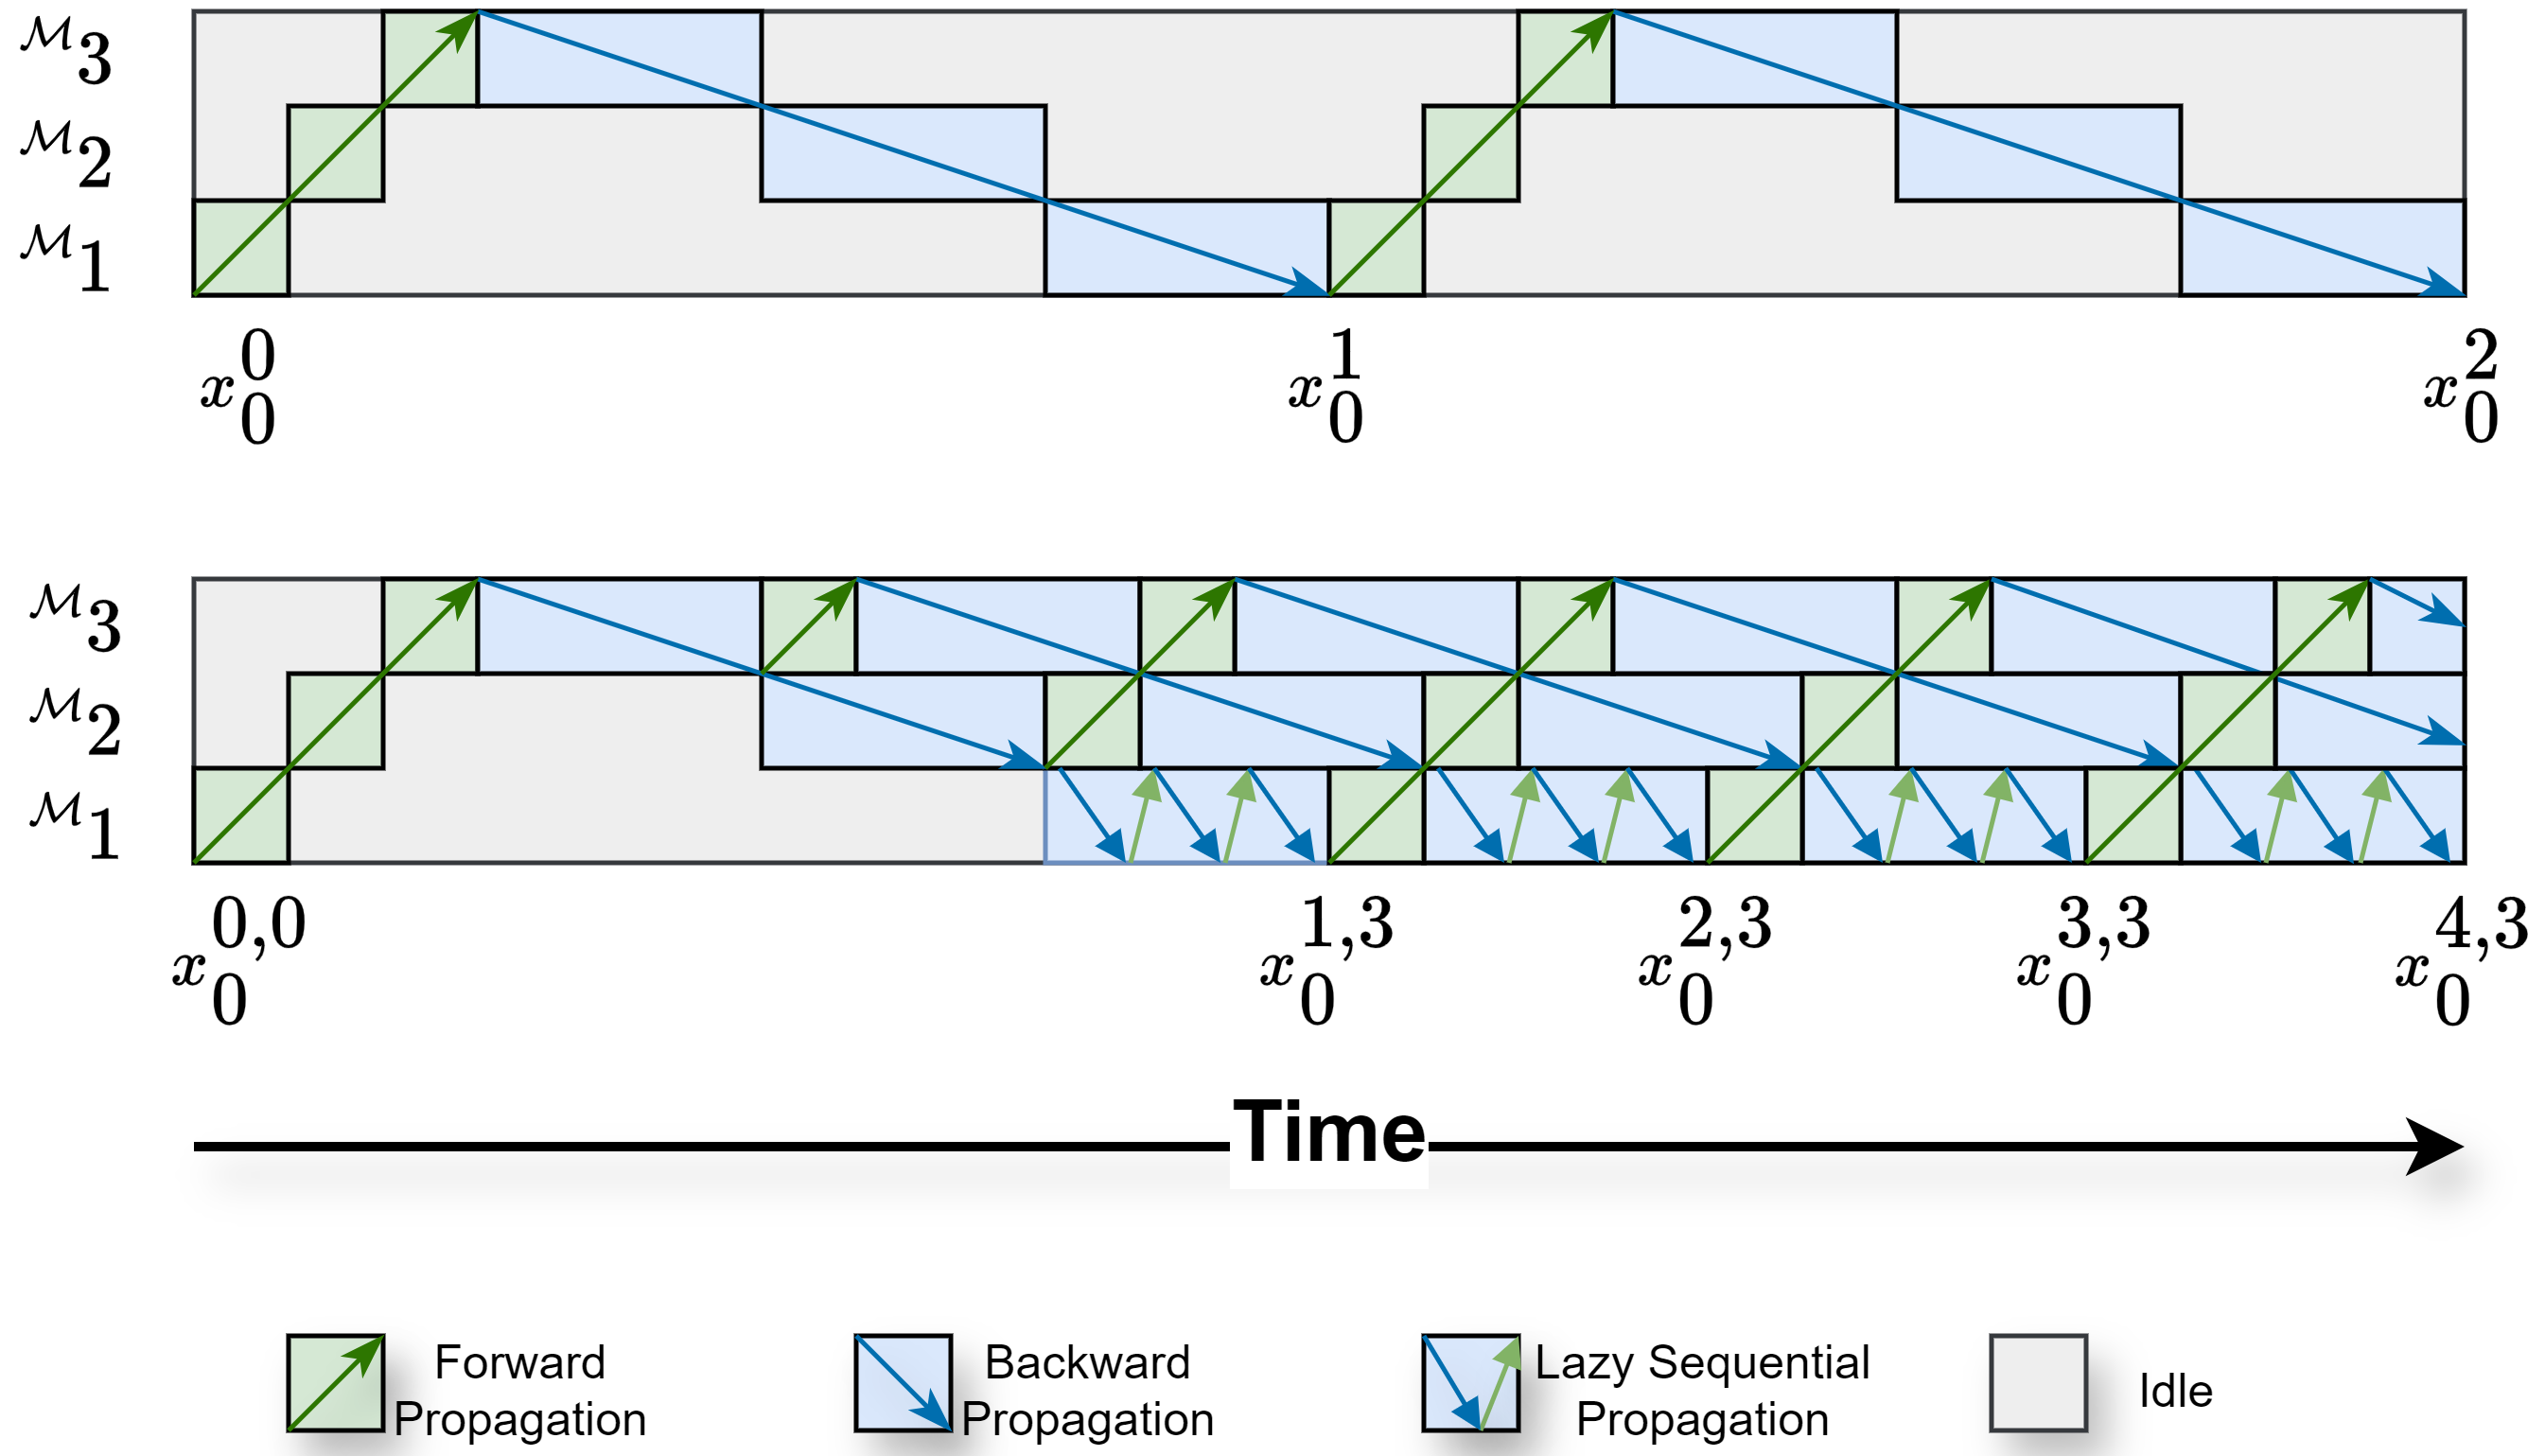
\includegraphics[width=0.5\linewidth]{pic/fig1-v3.png}
        % \end{center}
        \caption{Comparison of computation efficiency for adversarial sample updates.}
    \end{figure}
\end{frame}

\begin{frame}{Method}
    \begin{figure}[htpb]
        \centering
        % \begin{center}
        \includegraphics[width=\linewidth]{pic/fig2-0516.pdf}
        % \end{center}
        \caption{The conceptual comparison between VFAL with PGD (a) and DecVFAL (b).}
    \end{figure}
\end{frame}

\begin{frame}{Convergence Analysis}
\begin{figure}[htpb]
    \centering
    % \begin{center}
    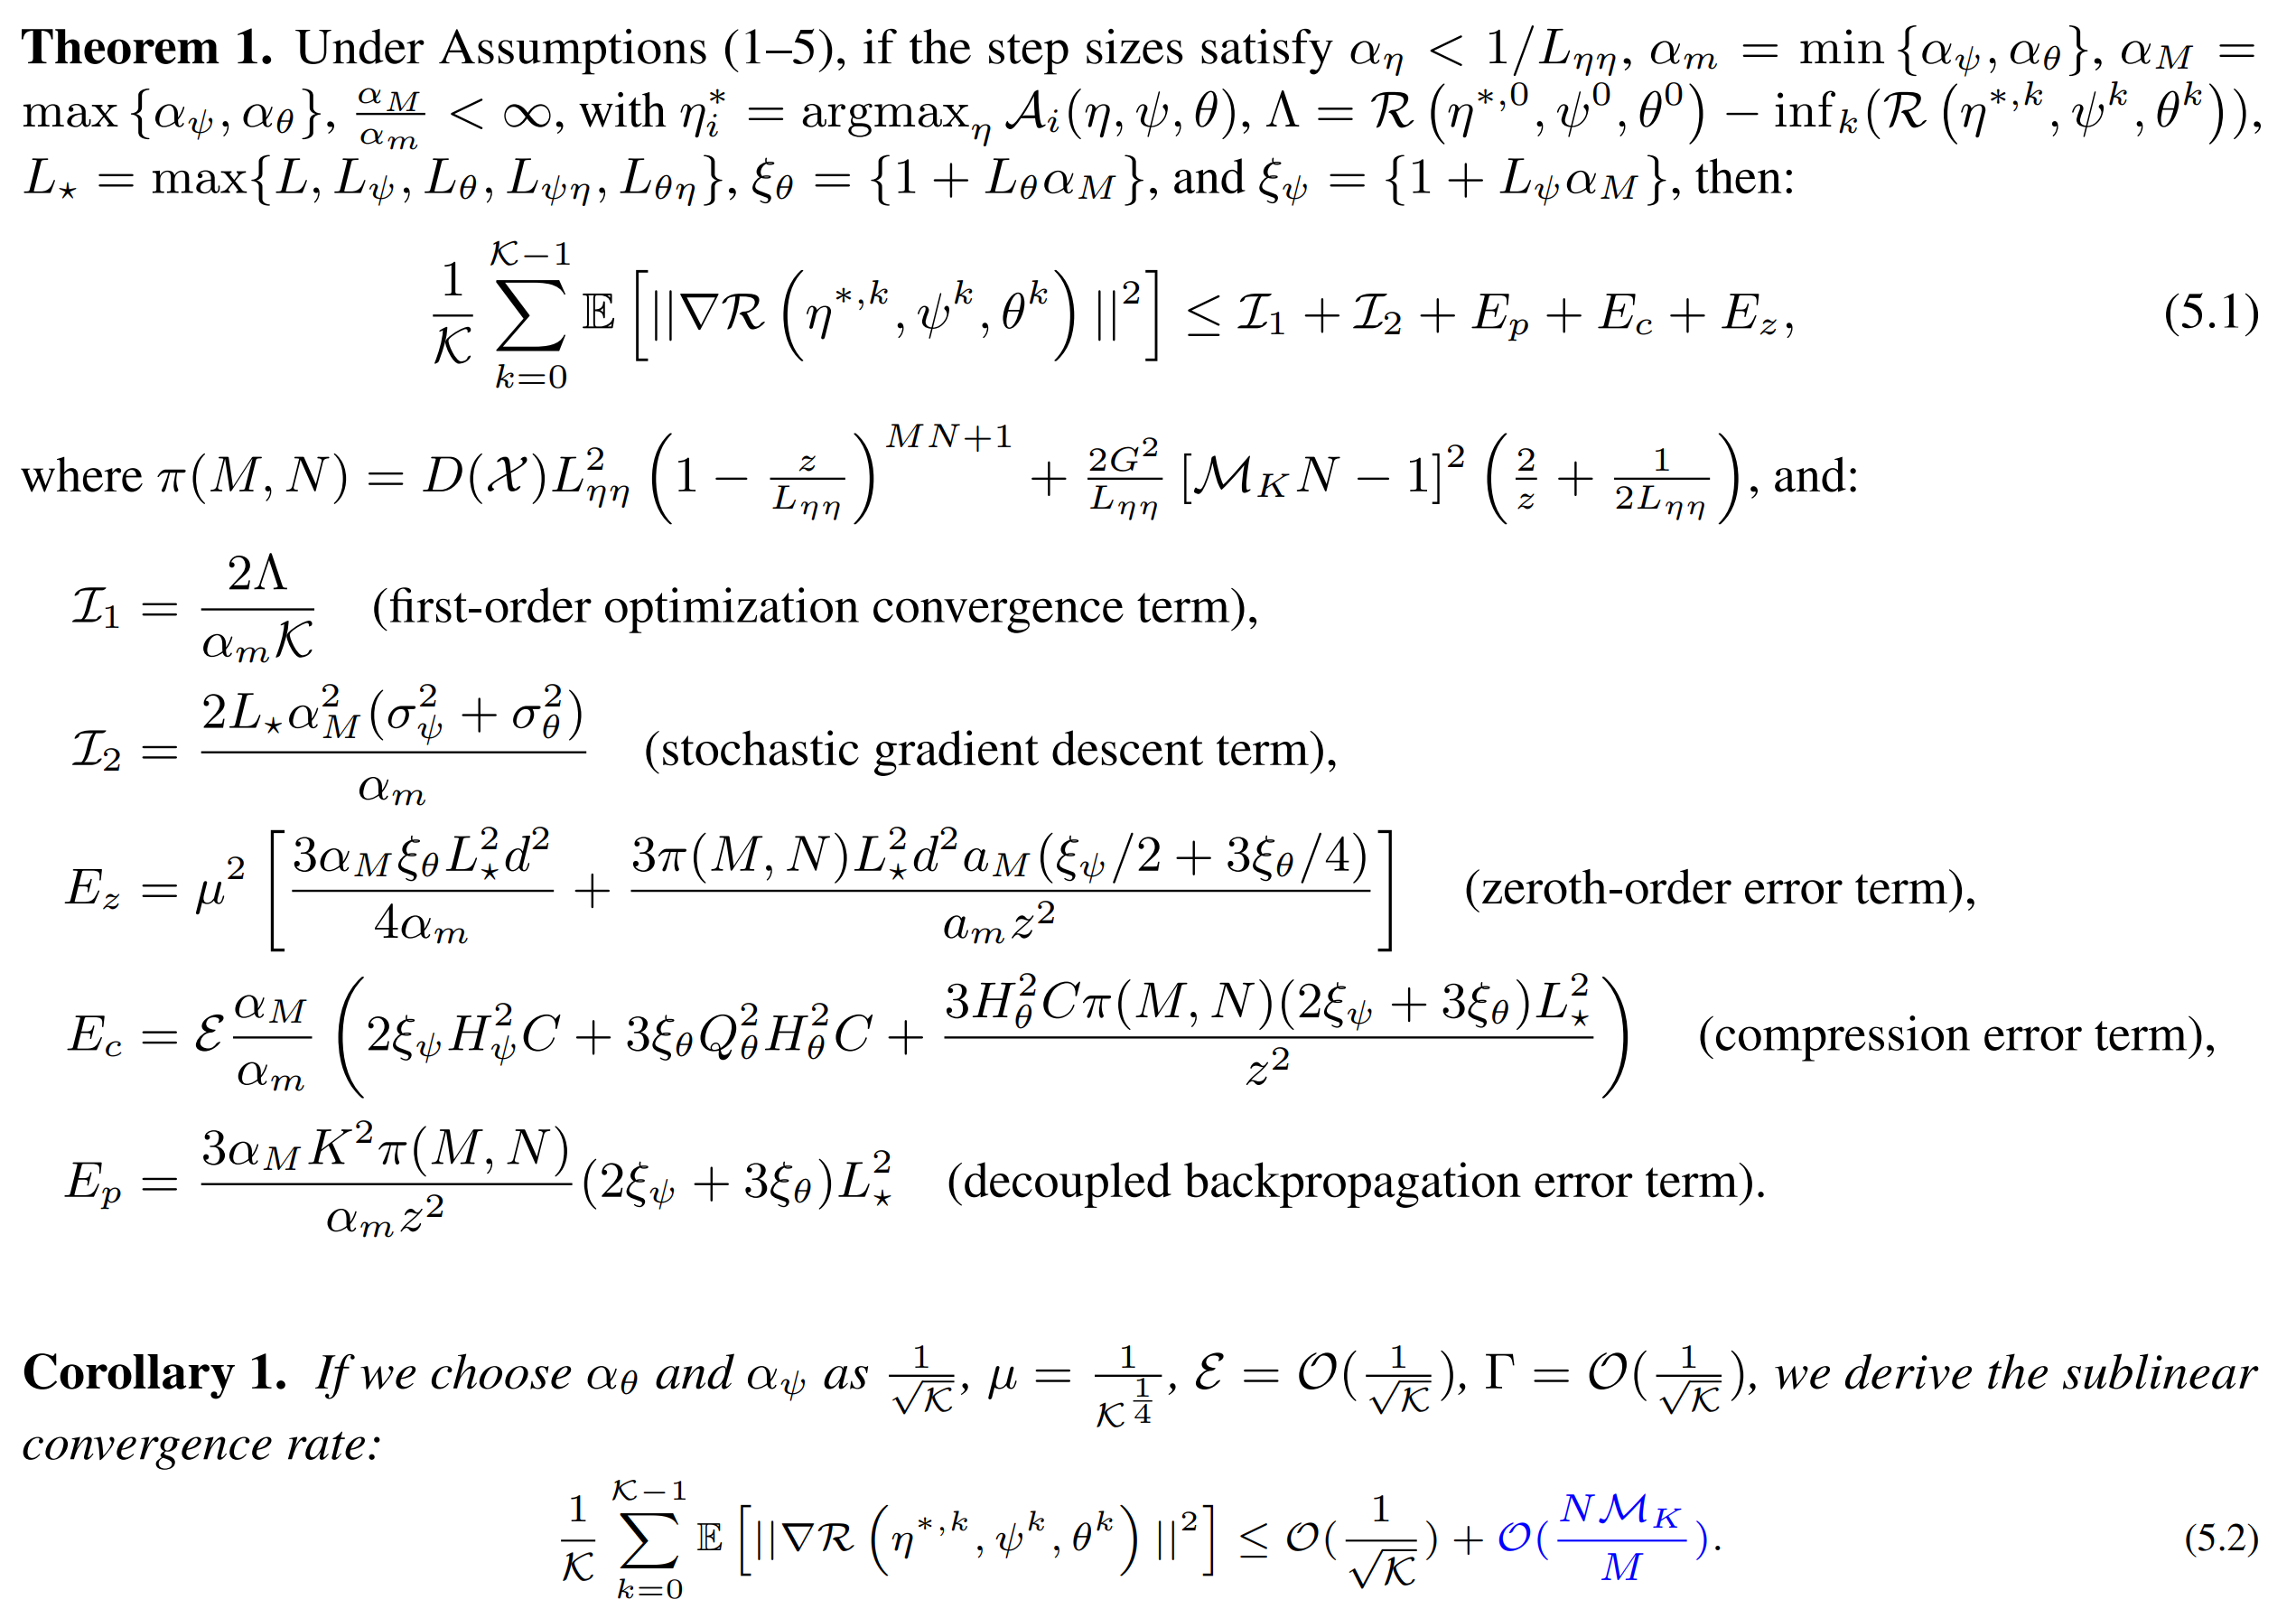
\includegraphics[width=0.8\linewidth]{pic/CA.png}
    % \end{center}
    % \caption{Convergence Analysis for  DecVFAL.}
\end{figure}
\end{frame}

\begin{frame}{Experiments}
\begin{figure}[htpb]
    \centering
    % \begin{center}
    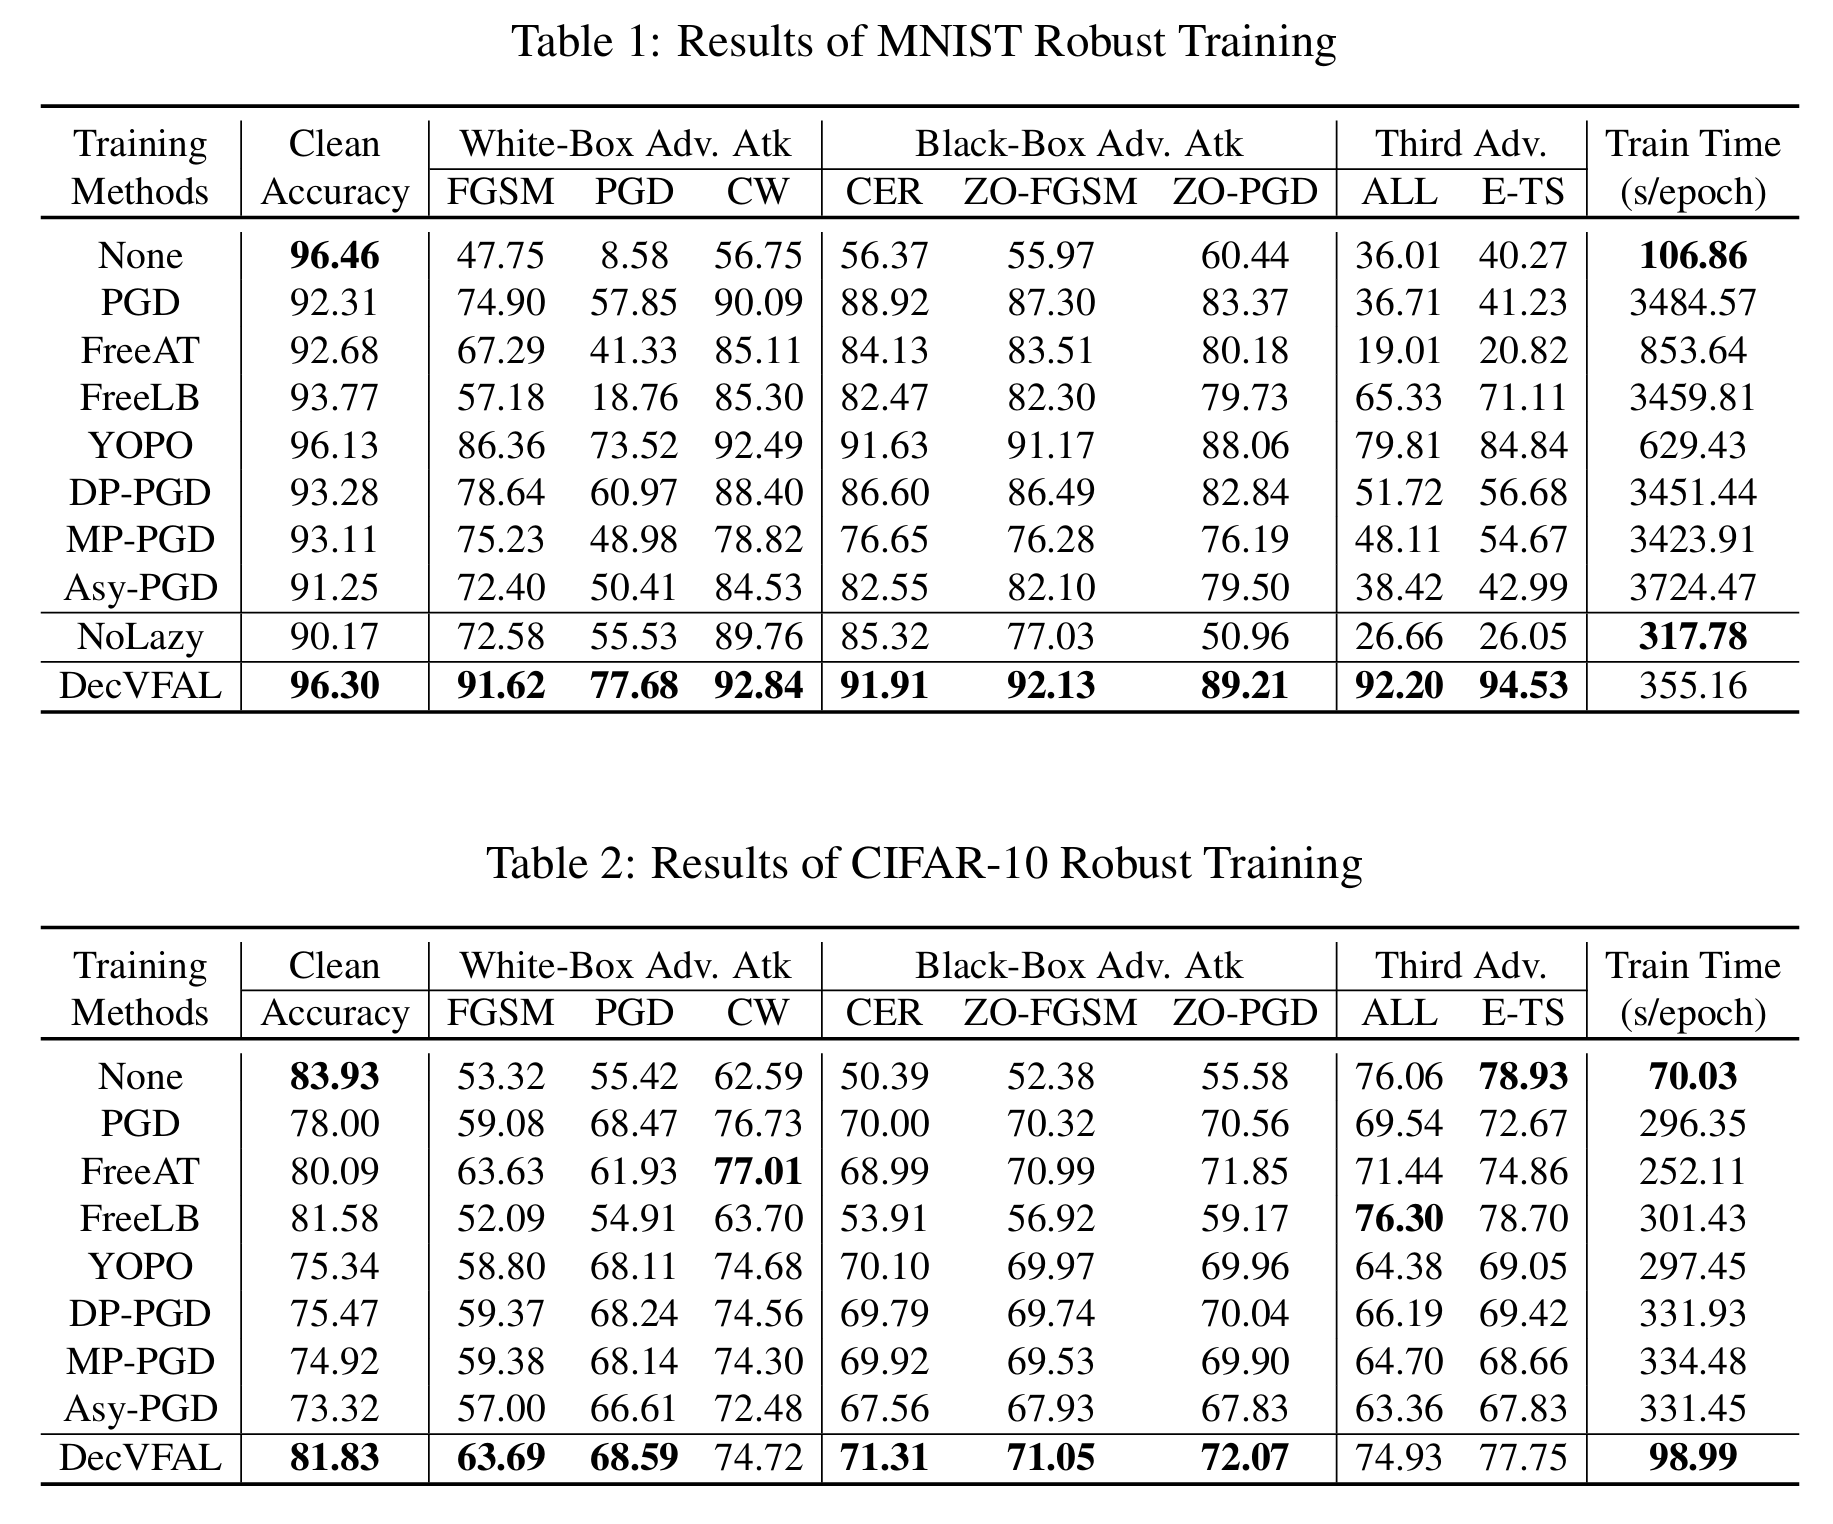
\includegraphics[width=0.75\linewidth]{pic/exp.png}
    % \end{center}
    % \caption{Convergence Analysis for  DecVFAL.}
\end{figure}
\end{frame}

\begin{frame}{Thanks}
    \begin{itemize}
        \item Paper: \\ https://neurips.cc/virtual/2025/loc/san-diego/poster/115884
        \item Code: \\ https://github.com/workelaina/DecVFAL
        \item Homepage: \\ https://workelaina.github.io/DecVFAL
    \end{itemize}
\end{frame}
\end{document}
